%===============================================================================
% LaTeX sjabloon voor de bachelorproef toegepaste informatica aan HOGENT
% Meer info op https://github.com/HoGentTIN/bachproef-latex-sjabloon
%===============================================================================

\documentclass{bachproef-tin}

\usepackage{hogent-thesis-titlepage} % Titelpagina conform aan HOGENT huisstijl
\usepackage{import}
\usepackage{pdfpages}
\usepackage{listings}
\lstset{
basicstyle=\small\ttfamily,
columns=flexible,
breaklines=true
}
\usepackage[dutch]{todonotes}

\import{../}{_variables.tex}

%%---------- Documenteigenschappen ---------------------------------------------
% TODO: Vul dit aan met je eigen info:

% De titel van het rapport/bachelorproef
\title{\bptitle}

% Je eigen naam
\author{\bpauthor}

% De naam van je promotor (lector van de opleiding)
\promotor{\bppromotor}

% De naam van je co-promotor. Als je promotor ook je opdrachtgever is en je
% dus ook inhoudelijk begeleidt (en enkel dan!), mag je dit leeg laten.
\copromotor{\bpcopromotor}

% Indien je bachelorproef in opdracht van/in samenwerking met een bedrijf of
% externe organisatie geschreven is, geef je hier de naam. Zoniet laat je dit
% zoals het is.
\instelling{Codifly}

% Academiejaar
\academiejaar{2021-2022}

% Examenperiode
%  - 1e semester = 1e examenperiode => 1
%  - 2e semester = 2e examenperiode => 2
%  - tweede zit  = 3e examenperiode => 3
\examenperiode{2}

%===============================================================================
% Inhoud document
%===============================================================================

\begin{document}

%---------- Taalselectie -------------------------------------------------------
% Als je je bachelorproef in het Engels schrijft, haal dan onderstaande regel
% uit commentaar. Let op: de tekst op de voorkaft blijft in het Nederlands, en
% dat is ook de bedoeling!

%\selectlanguage{english}

%---------- Titelblad ----------------------------------------------------------
\inserttitlepage

%---------- Samenvatting, voorwoord --------------------------------------------
\usechapterimagefalse
%%=============================================================================
%% Voorwoord
%%=============================================================================

\chapter*{\IfLanguageName{dutch}{Woord vooraf}{Preface}}
\label{ch:voorwoord}

%% TODO:
%% Het voorwoord is het enige deel van de bachelorproef waar je vanuit je
%% eigen standpunt (``ik-vorm'') mag schrijven. Je kan hier bv. motiveren
%% waarom jij het onderwerp wil bespreken.
%% Vergeet ook niet te bedanken wie je geholpen/gesteund/... heeft


% TODO Needs revision
Als ontwikkelaar vind ik het uitermate belangrijk om een goede kennis te hebben van waar je mee aan het werken bent, van het project zelf tot de individuele packages en libraries die je in gebruik neemt. React interesseerde me van de dag dat ik ervan hoorde, en na er een maand in een professionele omgeving mee gewerkt te hebben heb ik een hoog respect ontwikkeld voor hun ontwikkelaarsteam.

In de zoektocht naar de ideale developer experience ga ik op zoek naar de beste build tools die je kan gebruiken in een React project.

Zonder de steun van mijn vrienden en familie denk ik niet dat ik hier ooit zou geraakt zijn, daar zal ik ze eeuwig dankbaar voor zijn.
% TODO say something nice about your brother

%%=============================================================================
%% Samenvatting
%%=============================================================================

% TODO: De "abstract" of samenvatting is een kernachtige (~ 1 blz. voor een
% thesis) synthese van het document.
%
% Deze aspecten moeten zeker aan bod komen:
% - Context: waarom is dit werk belangrijk?
% - Nood: waarom moest dit onderzocht worden?
% - Taak: wat heb je precies gedaan?
% - Object: wat staat in dit document geschreven?
% - Resultaat: wat was het resultaat?
% - Conclusie: wat is/zijn de belangrijkste conclusie(s)?
% - Perspectief: blijven er nog vragen open die in de toekomst nog kunnen
%    onderzocht worden? Wat is een mogelijk vervolg voor jouw onderzoek?
%
% LET OP! Een samenvatting is GEEN voorwoord!

%%---------- Nederlandse samenvatting -----------------------------------------
%
% TODO: Als je je bachelorproef in het Engels schrijft, moet je eerst een
% Nederlandse samenvatting invoegen. Haal daarvoor onderstaande code uit
% commentaar.
% Wie zijn bachelorproef in het Nederlands schrijft, kan dit negeren, de inhoud
% wordt niet in het document ingevoegd.

%\IfLanguageName{english}{%
%\selectlanguage{dutch}
%\chapter*{Samenvatting}
%\lipsum[1-4]
%\selectlanguage{english}
%}{}

%%---------- Samenvatting -----------------------------------------------------
% De samenvatting in de hoofdtaal van het document

\chapter*{\IfLanguageName{dutch}{Samenvatting}{Abstract}}




%---------- Inhoudstafel -------------------------------------------------------
\pagestyle{empty} % Geen hoofding
\tableofcontents  % Voeg de inhoudstafel toe
\cleardoublepage  % Zorg dat volgende hoofstuk op een oneven pagina begint
\pagestyle{fancy} % Zet hoofding opnieuw aan

%---------- Lijst figuren, afkortingen, ... ------------------------------------

% Indien gewenst kan je hier een lijst van figuren/tabellen opgeven. Geef in
% dat geval je figuren/tabellen altijd een korte beschrijving:
%
%  \caption[korte beschrijving]{uitgebreide beschrijving}
%
% De korte beschrijving wordt gebruikt voor deze lijst, de uitgebreide staat bij
% de figuur of tabel zelf.

\listoffigures
\listoftables
\lstlistoflistings

% Als je een lijst van afkortingen of termen wil toevoegen, dan hoort die
% hier thuis. Gebruik bijvoorbeeld de ``glossaries'' package.
% https://www.overleaf.com/learn/latex/Glossaries

%---------- Kern ---------------------------------------------------------------

% De eerste hoofdstukken van een bachelorproef zijn meestal een inleiding op
% het onderwerp, literatuurstudie en verantwoording methodologie.
% Aarzel niet om een meer beschrijvende titel aan deze hoofstukken te geven of
% om bijvoorbeeld de inleiding en/of stand van zaken over meerdere hoofdstukken
% te verspreiden!

%%=============================================================================
%% Inleiding
%%=============================================================================

\chapter{\IfLanguageName{dutch}{Inleiding}{Introduction}}
\label{ch:inleiding}

De inleiding moet de lezer net genoeg informatie verschaffen om het onderwerp te begrijpen en in te zien waarom de onderzoeksvraag de moeite waard is om te onderzoeken. In de inleiding ga je literatuurverwijzingen beperken, zodat de tekst vlot leesbaar blijft. Je kan de inleiding verder onderverdelen in secties als dit de tekst verduidelijkt. Zaken die aan bod kunnen komen in de inleiding~\autocite{Pollefliet2011}:

\begin{itemize}
  \item context, achtergrond
  \item afbakenen van het onderwerp
  \item verantwoording van het onderwerp, methodologie
  \item probleemstelling
  \item onderzoeksdoelstelling
  \item onderzoeksvraag
  \item \ldots
\end{itemize}

Er zijn 

\section{\IfLanguageName{dutch}{Probleemstelling}{Problem Statement}}
\label{sec:probleemstelling}

Uit je probleemstelling moet duidelijk zijn dat je onderzoek een meerwaarde heeft voor een concrete doelgroep. De doelgroep moet goed gedefinieerd en afgelijnd zijn. Doelgroepen als ``bedrijven,'' ``KMO's,'' systeembeheerders, enz.~zijn nog te vaag. Als je een lijstje kan maken van de personen/organisaties die een meerwaarde zullen vinden in deze bachelorproef (dit is eigenlijk je steekproefkader), dan is dat een indicatie dat de doelgroep goed gedefinieerd is. Dit kan een enkel bedrijf zijn of zelfs één persoon (je co-promotor/opdrachtgever).

\section{\IfLanguageName{dutch}{Onderzoeksvraag}{Research question}}
\label{sec:onderzoeksvraag}

Wees zo concreet mogelijk bij het formuleren van je onderzoeksvraag. Een onderzoeksvraag is trouwens iets waar nog niemand op dit moment een antwoord heeft (voor zover je kan nagaan). Het opzoeken van bestaande informatie (bv. ``welke tools bestaan er voor deze toepassing?'') is dus geen onderzoeksvraag. Je kan de onderzoeksvraag verder specifiëren in deelvragen. Bv.~als je onderzoek gaat over performantiemetingen, dan 

\section{\IfLanguageName{dutch}{Onderzoeksdoelstelling}{Research objective}}
\label{sec:onderzoeksdoelstelling}

Wat is het beoogde resultaat van je bachelorproef? Wat zijn de criteria voor succes? Beschrijf die zo concreet mogelijk. Gaat het bv. om een proof-of-concept, een prototype, een verslag met aanbevelingen, een vergelijkende studie, enz.

\section{\IfLanguageName{dutch}{Opzet van deze bachelorproef}{Structure of this bachelor thesis}}
\label{sec:opzet-bachelorproef}

% Het is gebruikelijk aan het einde van de inleiding een overzicht te
% geven van de opbouw van de rest van de tekst. Deze sectie bevat al een aanzet
% die je kan aanvullen/aanpassen in functie van je eigen tekst.

De rest van deze bachelorproef is als volgt opgebouwd:

In Hoofdstuk~\ref{ch:stand-van-zaken} wordt een overzicht gegeven van de stand van zaken binnen het onderzoeksdomein, op basis van een literatuurstudie.

In Hoofdstuk~\ref{ch:methodologie} wordt de methodologie toegelicht en worden de gebruikte onderzoekstechnieken besproken om een antwoord te kunnen formuleren op de onderzoeksvragen.

% TODO: Vul hier aan voor je eigen hoofstukken, één of twee zinnen per hoofdstuk

In Hoofdstuk~\ref{ch:conclusie}, tenslotte, wordt de conclusie gegeven en een antwoord geformuleerd op de onderzoeksvragen. Daarbij wordt ook een aanzet gegeven voor toekomstig onderzoek binnen dit domein.
\chapter{\IfLanguageName{dutch}{Stand van zaken}{State of the art}}
\label{ch:stand-van-zaken}

% Tip: Begin elk hoofdstuk met een paragraaf inleiding die beschrijft hoe
% dit hoofdstuk past binnen het geheel van de bachelorproef. Geef in het
% bijzonder aan wat de link is met het vorige en volgende hoofdstuk.

% Pas na deze inleidende paragraaf komt de eerste sectiehoofding.

% Dit hoofdstuk bevat je literatuurstudie. De inhoud gaat verder op de inleiding, maar zal het onderwerp van de bachelorproef *diepgaand* uitspitten. De bedoeling is dat de lezer na lezing van dit hoofdstuk helemaal op de hoogte is van de huidige stand van zaken (state-of-the-art) in het onderzoeksdomein. Iemand die niet vertrouwd is met het onderwerp, weet nu voldoende om de rest van het verhaal te kunnen volgen, zonder dat die er nog andere informatie moet over opzoeken \autocite{Pollefliet2011}.

% Je verwijst bij elke bewering die je doet, vakterm die je introduceert, enz. naar je bronnen. In \LaTeX{} kan dat met het commando \texttt{$\backslash${textcite\{\}}} of \texttt{$\backslash${autocite\{\}}}. Als argument van het commando geef je de ``sleutel'' van een ``record'' in een bibliografische databank in het Bib\LaTeX{}-formaat (een tekstbestand). Als je expliciet naar de auteur verwijst in de zin, gebruik je \texttt{$\backslash${}textcite\{\}}.
% Soms wil je de auteur niet expliciet vernoemen, dan gebruik je \texttt{$\backslash${}autocite\{\}}. In de volgende paragraaf een voorbeeld van elk.

% \textcite{Knuth1998} schreef een van de standaardwerken over sorteer- en zoekalgoritmen. Experten zijn het erover eens dat cloud computing een interessante opportuniteit vormen, zowel voor gebruikers als voor dienstverleners op vlak van informatietechnologie~\autocite{Creeger2009}.

% \lipsum[7-20]

Om van slag te gaan met de bundlers en transpilers, is het handig om ook eerst even stil te staan bij de installatie, en hoe die verloopt.

\todo[inline]{TODO: Deze inleiding beter maken, doorvloeien eenmaal de inleiding af is}

\section{npm en Yarn}

Wanneer er aan een Node project gewerkt wordt, zal er waarschijnlijk gebruik gemaakt worden van npm. npm staat voor Node Package Manager, en zoals de naam impliceert is npm een tool om JavaScript-libraries binnen je project te beheren. Alle projecten die hieronder besproken zullen worden zijn dan ook beschikbaar op \href{https://www.npmjs.com/}{de npm-website}.

\subsection{Initialisatie}

Een nieuw npm-project kan geïnitialiseerd worden aan de hand van het ``\lstinline{npm init}'' commando. Wanneer hier geen verdere argumenten aan gegeven worden zal dit een alleen een package.json bestand aanmaken. De package.json kan de volgende elementen bevatten: \autocite{npmDocsPackageJson}

\begin{itemize}
    \item Algemene informatie over het project (versie, auteur, naam \ldots). Dit is vooral relevant als het project bedoeld is om zelf op npm beschikbaar te worden.
    \item Een verzameling van commando's die uitvoerbaar zijn aan de hand van ``\lstinline{npm run [naam van commando]}''
    \item De verzameling van packages waarvan dit project afhankelijk is.
    \item De versie van node die dit project gebruikt.
    \item Nog een aantal andere parameters die niet relevant zijn voor dit onderzoek (OS, CPU \ldots).
\end{itemize}

Verder kan ook een initializer meegegeven worden aan het init-commando. Een initializer is een npm project dat als prefix ``create-'' heeft, en bevat alle scaffolding die nodig is voor dat bepaald soort project. \lstinline{create-react-app} zal bijvoorbeeld al de startbestanden voor een React app bevatten, en de nodige dependencies om direct aan de slag te kunnen gaan.

\subsection{Dependencies}

Zoals hiervoor vernoemd, bevat de package.json een verzameling van packages waarvan het project afhankelijk is. Deze worden de ``dependencies'' genoemd. Er zijn 5 verschillende soorten dependencies, waarvan de volgende 3 relevant zijn om uit te leggen:

\subsubsection{Normale Dependencies}

Dit is de standaardmanier waarop dependencies toegevoegd worden door npm. Een normale dependency wordt toegevoegd aan de hand van het ``\lstinline{npm i [package]}'' commando. Deze dependencies worden ook meegeleverd in het eindproduct voor de consument. Dit zijn dus functionele benodigdheden bij de uitvoering van het project in een productie-omgeving.

\subsubsection{Development Dependencies}

Het wordt aangeraden om packages die niet nodig zijn om het project uit te voeren binnen een productie-omgeving te installeren als ``devdependency''. Dit wordt gedaan aan de hand van het ``\lstinline{npm i -D [package]}'' commando. Dependencies die als devdependency toegevoegd worden zullen dus niet meegeleverd worden bij het eindproduct, wat de totale grootte van het project kleiner houdt. Bundlers en transpilers vallen onder deze categorie, aangezien het transpileer- en bundelproces deel zijn van wat er moet gebeuren \emph{voor} dat het eindproduct in de productieomgeving wordt geplaatst.

\subsubsection{Peer Dependencies}

Alle packages op npm zijn zelf ook npm-projecten. Dit betekent dus dat zij ook allemaal een package.json hebben, en afhankelijk zijn van bepaalde packages. Een peer dependency is een dependency die niet door de ontwikkelaar zelf wordt toegevoegd, maar door een andere package die de ontwikkelaar toegevoegd heeft.

Het is dus makkelijk om zich voor te stellen dat dit na een tijd leidt naar heel veel dependencies. Gelukkig doet npm aan ``dependency resolution'', waar zoveel mogelijk duplicate dependencies en conflicten opgelost worden.

\subsection{Yarn}

npm is niet de enige package manager. Één van de andere opties is Yarn. Yarn werkt op veel vlakken op een gelijkaardige manier. Beiden tools bestaan voor dezelfde doeleinden, en gebruiken de npm repository om hun packages op te halen. Waar Yarn wél licht in verschilt is hoe het omgaat met het installeren van packages, en het dependency resolution proces. Yarn installeert alle packages in parallel, wat resulteert in veel een sneller installatieproces vergeleken met de synchrone installatie van npm. Op het vlak van dependency resolution is Yarn iets consistenter. Yarn kijkt naar de versie-definitie, terwijl npm kijkt naar de de eigenlijke versie. \autocite{Kay2021} \todo[inline]{TODO: Wat meer info geven over de versie-definities.}

Binnen Codifly wordt altijd Yarn gebruikt, en alle experimenten zullen ter gevolge ook via Yarn uitgevoerd worden. Als een Yarn-commando gebruikt wordt zal de npm-equivalent ook toegelicht worden.

\section{Bundlers}

Bundlers hebben als doel je modulaire JavaScript-code samen te bundelen in 1 bestand voor consumptie op het web. In het verleden konden browsers niet verschillende modules inladen, en hoewel dat nu wel vaak het geval is, heeft het nog steeds zijn voordelen. HTTP/2 biedt browsers de mogelijkheid aan om veel meer dan de hiervoor traditionele 6 verbindingen met een server te openen. Dit is goed als er veel verschillende modules ingeladen moeten worden, maar het lost niet alles op. De browser moet nog steeds 1 per 1 de boom van dependencies afgaan, en pas wanneer er een nieuwe dependency gevonden wordt, wordt die opgevraagd. Ook compressie is minder efficiënt in vele kleinere chunks dan één grote bundel. \autocite{you_2021} Verder is er ook het probleem dat veel externe packages, hoewel ze in ESM syntax geschreven worden, gepubliceerd worden in CJS formaat. CJS formaat is echter niet leesbaar door browsers zonder hulp van een library zoals RequireJS. \autocite{sweeney_2020}

Een bundler bereikt dit door via het ingangspunt van je JavaScript alles te scannen, wanneer de bundler een nieuwe import tegenkomt zal die ook daardoor gaan. Dit proces noemt het bouwen van de dependency graph. Op basis daarvan zal de bundler weten wat er allemaal toegevoegd zal moeten worden aan de bundel.

Er zijn veel opties voor het bundelen van JavaScript in een project. Elke bundler heeft echter wel een aantal configuratie-opties die in de ene of andere vorm ook aanwezig zijn in alle andere bundlers.

\subsection{Grotendeels Universele Features}

Om te weten wat er gebundeld moet worden, moet er een ingangspunt aanwezig zijn. Dit kan 1 JavaScript bestand zijn of meerderen. Sommige bundlers ondersteunen ook een HTML bestand als ingangspunt, maar functioneel biedt dit geen voordeel. \todo[inline]{TODO: Bron}
Sommige bundlers, vooral de bundlers die als zero-configuration worden geadverteerd, zullen ook automatisch een ingangspunt veronderstellen als ze niet expliciet is meegegeven (Meestal ``\lstinline{./public/index.js}'').

Als er een ingangspunt is, is er ook een uitgangspunt. Dit kan een enkel bestand zijn, of een folder voor meerdere bestanden.

Bundlers hebben gewoonlijks ook ondersteuning voor plugins. Plugins bieden een extra functionaliteit die de bundler zelf niet levert. Meestal vallen dingen zoals de compressie van afbeeldingen of ESLint validatie hieronder.

Het is ook mogelijk om te onderscheiden tussen de verschillende omgevingen waarin gebundeld wordt, zijnde meestal development, staging en productie. Het kan bijvoorbeeld zijn dat er in een bepaalde omgeving geen nood is aan een bepaald plugin. Standaard is er al een onderscheiding tussen development en productie, waar de productiebuilds dan geen formattering zullen toepassen die normaliter het ontwikkelingsproces vergemakkelijken.

\subsection{De No-bundler Movement}

Bepaalde bundlers, zoals Vitejs, opteren om in een developmentomgeving de bronbestanden niet meer samen te bundelen. Dit betekent niet dat er geen bundler meer nodig is, maar in de plaats daarvan worden de bestanden door de bundler getransformeerd in chunks die moderne browser kunnen interpreteren. Dit zorgt ervoor dat naast de devserver opstarten, er niet al te veel meer moet gebeuren. De tijd om de server te starten zou dan tot 100x minder lang kunnen duren, in enkele seconden of minder. De individuele chunks worden dan ook gecached door de browser, wat betekent dat als er veranderingen gebeuren alleen maar de aangepaste chunks opnieuw geladen moeten worden. Dit is wat in de praktijk HMR, of hot module replacement genoemd wordt. Veel bundlers ondersteunen HMR, maar vaak niet out-of-the-box. Zo niet, kan het ook lastig zijn om werkende te krijgen. \todo[inline]{TODO: Bron}

\missingfigure{TODO: populariteitsgraph van bundlers}

\subsection{De lijst}

In dit onderzoek zal vooral naar de volgende bundlers gekeken worden:

\subsubsection{Webpack}

De populairste en één van de eerdere bundlers in gebruik vandaag is Webpack. Bij veel project-templates wordt Webpack meegeleverd als de standaardbundler. Bij een blanco project kan deze echter ook toegevoegd worden met \lstinline{npm i -D webpack}. Webpack heeft goede ondersteuning en veel plugins om het bundelingsproces te vergemakkelijken. Door de ouderdom van Webpack is er echter veel dat ondersteund moet worden, wat ook nadelen met zich meebrengt. De configuratie voelt onhandig en moeilijk te lezen aan, door de hoeveelheid verschillende plugins nodig zijn om bepaalde taken te bereiken. De syntax van de configuratie is in het algemeen ook niet met te veel ontwikkelaarsvriendelijkheid over termijn in gedachte gemaakt, wat ons naar de volgende optie brengt.

\subsubsection{Rollup}

Rollup is een bundler die zich veel meer focust op productie builds. Webpack doet bijna alles voor een ontwikkelaar. Het bevat standaard een dev server, en kan met veel meer dan alleen JavaScript omweg. Rollup focust zich geheel op het bundelen van de JavaScript op een zo efficiënt mogelijke manier, maar als gevolg heeft Rollup weinig te bieden voor ontwikkelaars tijdens het ontwikkelen zelf. Ook al is de configuratie in het algemeen korter dan Webpack.

\subsubsection{Vitejs}

Vite is een bundler die ontwikkeld is door Evan You, de maker van Vue. Vite is geadverteerd als een zero-configuration bundler die deel is van de no-bundler movement. Onderliggend gebruikt Vite standaard ESBuild om JavaScript en TypeScript te transpileren en bundelen. Dit is echter alleen in een ontwikkelingsomgeving. ESBuild bevat nog niet alle functionaliteit om bruikbaar te zijn in een productieomgeving. In plaats van ESBuild gebruikt Vite Rollup voor productie builds. \autocite{you_2021}

\subsubsection{Parcel}

Parcel is ook een zero-configuration bundler, maar is volledig geschreven met Rust. Onderliggend gebruikt het SWC om JavaScript en TypeScript te transpileren. SWC is een transpiler in Rust geschreven, die een heel goede performantie heeft vergeleken met de met traditionele transpilers. Naast dit is het grootste verschil tussen de 2 dat Parcel wel nog alles bundelt in de ontwikkelingsomgeving. Parcel heeft ook zijn eigen CSS compiler, wat verdere voordelen voor performantie biedt. \autocite{dahan_2021}

\subsubsection{ESBuild}

ESBuild is de jongste bundler die hier vergeleken wordt. Hoewel ESBuild momenteel nog niet aan zijn v1.0.0 release is, is de performantie zeer veelbelovend. ESBuild is geschreven in Go, en is natively compiled per platform. Dit in combinatie met een asynchrone werkwijze zorgt voor een heel goede performantie, die alleen geëvenaard wordt door SWC. Dat is te danken aan hun focus op snelheid en keuze van talen. Rust en Go zijn veel meer performant dan een JavaScript-omgeving kan zijn. \autocite{eaton_2021}

Hoewel ESBuild zeer snel is, is het door zijn jonge leeftijd ook de meest gebrekkige qua features. HMR en code-splitting zijn bijvoorbeeld nog niet geïmplementeerd. \autocite{wallace}

\section{Transpilers}

Transpilers hebben enerzijds als doel de moderne JavaScript die we schrijven om te zetten naar een versie van ECMAScript dat ondersteund wordt door de meeste browsers. Anderzijds kunnen ze ook TypeScript transpileren naar JavaScript. \todo[inline]{TODO: Iets meer info over hoe transpilers werken}

Hoewel elke bundler theoretisch via een plugin elke onafhankelijke transpiler kan gebruiken, is een grote vraag in dit onderzoek of dit de moeite waard is bij alle bundlers. Parcel werkt bijvoorbeeld standaard met SWC. Als Webpack gecombineerd zou worden met SWC, zou de performantie dicht kunnen komen bij die van Parcel? Het bundelen zelf duurt ook nog even, dus het is ook perfect mogelijk dat de tijd gewonnen met SWC als transpiler te gebruiken in Webpack niks is in vergelijking met de gecombineerde snelheid van Parcel en SWC.

\subsection{TSC}

TSC is de standaardtranspiler die met TypeScript komt. Het biedt typechecking aan, waar enige fouten in de TypeScript typering gemeld zullen worden en de transpilatie zullen afbreken.

\begin{lstlisting}
const exampleValue: string = 5;
\end{lstlisting}

Deze code zal TSC niet kunnen compileren, aangezien 5 geen string is.

De performantie van TSC is niets speciaal, de typechecking introduceert ook een grote overhead.

\subsection{Babel}

Babel is de meest uitbreidbare transpiler in deze lijst. Er zijn veel plugins beschikbaar om de nieuwste ES proposals te ondersteunen, of om andere syntaxes zoals JSX of Flow te ondersteunen.

Babel is de minst performante van de opties. Het is ook de oudste en net zoals Webpack heeft dat gevolgen gehad op de complexiteit en performantie doorheen de jaren. \todo[inline]{TODO: Bron}

\subsection{Sucrase}

Sucrase is een fork van Babel die bedoeld is om te transpileren naar recente versies van ECMAScript, en zijn focus vooral legt naar het ondersteunen van andere extensies op JavaScript, zoals JSX, TypeScript en Flow. Hierdoor is Sucrase minder uitbreidbaar, maar heel wat sneller. \autocite{pierce}

\subsection{SWC}

SWC is zoals hiervoor vernoemd de standaardtranspiler van Parcel, in Rust geschreven. SWC maakt gebruik van parallellisatie en een performante taal om potentieel meer dan 70x sneller te zijn dan Babel. \autocite{swc}

\todo[inline]{TODO: Meer details over transpilers, meer bronnen citeren}

%%=============================================================================
%% Methodologie
%%=============================================================================

\chapter{\IfLanguageName{dutch}{Methodologie}{Methodology}}
\label{ch:methodologie}

%% TODO: Hoe ben je te werk gegaan? Verdeel je onderzoek in grote fasen, en
%% licht in elke fase toe welke stappen je gevolgd hebt. Verantwoord waarom je
%% op deze manier te werk gegaan bent. Je moet kunnen aantonen dat je de best
%% mogelijke manier toegepast hebt om een antwoord te vinden op de
%% onderzoeksvraag.

Om te kunnen achterhalen welke combinatie van bundler en transpiler beide een efficiënte en betrouwbare keuze zou zijn voor gebruik binnen Codifly, zijn er de volgende overwegingen die gemaakt moesten gemaakt worden:

\section{Wat wilt Codifly?}

Hier kan er onderscheid gemaakt worden tussen 2 categorieën: Het belang van de business, en het belang van de ontwikkelaar. Een ideale oplossing zou beiden de business en ontwikkelaars tevreden houden.

\subsection{De Noden van de Ontwikkelaars}

Om te peilen wat voor technische features aanwezig zouden moeten zijn, is de onderzoeker van plan een anonieme vragenlijst te presenteren aan de ontwikkelaar binnen Codifly. Deze vragenlijst zal de volgende vragen bevatten:

\begin{itemize}
    \item Een verzameling van veelvoorkomende features in bundlers, met als vraag een ordinale score van 1 tot en met 6 te geven op het belang van die feature.
    \begin{description}
        \item[Mogelijke antwoorden:] \hfill
        \begin{enumerate}
            \item Ik weet het niet / Ik ben niet zeker
            \item Helemaal niet belangrijk
            \item Niet belangrijk
            \item Heeft toepassingen
            \item Zeer belangrijk
            \item Dit is essentieel
        \end{enumerate}
        \item[Features:] \hfill
        \begin{itemize}
            \item Code-splitting
            \item Zero-configuration
            \item High speed bundling
            \item Customisability
            \item ES5 Support
            \item Dynamic expressions in import
            \item Typescript typechecking
            \item Hot module replacement
        \end{itemize}
    \end{description}
    \item Optionele andere feature(s) waar de ontwikkelaar belang aan hecht.
    \item Andere opmerkingen
\end{itemize}

\todo[inline]{TODO: de features hierboven ook zeker allemaal coveren in lit. studie}

\subsection{De Noden van de Business}

De voornaamste zorg vanuit het business-aspect is de configuratie van de bundler. Vaak kan er veel tijd gegoten worden in het oplossen van bepaalde problemen die gerelateerd zijn aan de configuratie van Webpack. Daarom is het volgens Arvid, één van de bedrijfsleiders van Codifly en de co-promotor van deze paper, het belangrijkste aspect in de keuze van bundler.

Performantie is in de ogen van de business iets minder belangrijk dan de configuratie.

\todo[inline]{TODO: is dit zelfs passend bij methodologie? Moet het niet bij conclusie?}

Codifly richt zich voornamelijk op een ``one-size-fits-all'' oplossing. Er bestaat een seed-project dat een project-template bijhoudt voor gebruik in de meeste nieuwe projecten.

Een snelle opstart met een voorgedefinieerde configuratie of minimale configuratie is als gevolg een belangrijke metric.

\section{Praktische Testen}

Om kwantitatieve resultaten te behalen heeft de onderzoeker de keuze genomen de performantie van een aantal reële en niet-reële projecten te meten met de onder dit onderzoek gestaafde bundlers. Omdat de huidige React-projecten binnen Codifly allemaal Webpack gebruiken, zal Webpack ook voornamelijk dienen als referentie in deze testen.

\subsection{De Gebruikte Projecten}

Er zal hier een onderscheid zijn tussen reële projecten en niet-reële projecten. Voor praktische redenen, zoals de tijd die het kan nemen om een dergelijke migratie uit te voeren, zal er een mix zijn van projecten die bestaan binnen Codifly en projecten die puur voor variatie aanwezig zijn.

\subsubsection{Interne Projecten}

De primaire motivatie achter deze keuzes is dat de onderzoeker al dergelijke kennis heeft van deze projecten, wat het proces van het migreren zal vergemakkelijken.

De volgende interne projecten van Codifly zullen aangekaart worden:

\paragraph{De corporate website van Codifly}

De website van Codifly, beschikbaar op \href{https://www.codifly.be}{www.codifly.be}. Dit project is in 2021 herwerkt van JavaScript + Flow naar Typescript. Als resultaat is dit een vrij moderne codebase om mee te werken, wat een goed beeld geeft op hoe de bundlers zouden omgaan met een nieuw project.

Ook een voor- en nadeel is het feit dat er geen complexe API-calls uitgevoerd worden. Het enige waar dat in het project voor nodig is, is voor de inzendingen van een formulier via mail. Dit betekent dus enerzijds dat de migratie naar verschillende bundlers minder op conflicten zou mogen stuiten, maar anderzijds geeft dit dan ook een minder goed beeld op de interacties met API-projecten.

\paragraph{Het webplatform van Depannage Steps}

\todo[inline]{TODO: Pretty sure dat DS een te lage nodejs versie gebruikt om vite en esbuild te testen, verify this.}

% Voeg hier je eigen hoofdstukken toe die de ``corpus'' van je bachelorproef
% vormen. De structuur en titels hangen af van je eigen onderzoek. Je kan bv.
% elke fase in je onderzoek in een apart hoofdstuk bespreken.

%\input{...}
%\input{...}
%...

%%=============================================================================
%% Conclusie
%%=============================================================================

\chapter{Conclusie}
\label{ch:conclusie}

% TODO: Trek een duidelijke conclusie, in de vorm van een antwoord op de
% onderzoeksvra(a)g(en). Wat was jouw bijdrage aan het onderzoeksdomein en
% hoe biedt dit meerwaarde aan het vakgebied/doelgroep? 
% Reflecteer kritisch over het resultaat. In Engelse teksten wordt deze sectie
% ``Discussion'' genoemd. Had je deze uitkomst verwacht? Zijn er zaken die nog
% niet duidelijk zijn?
% Heeft het onderzoek geleid tot nieuwe vragen die uitnodigen tot verder 
%onderzoek?

\lipsum[76-80]



%%=============================================================================
%% Bijlagen
%%=============================================================================

\appendix
\renewcommand{\chaptername}{Appendix}

\chapter{Vragenlijst Developers}

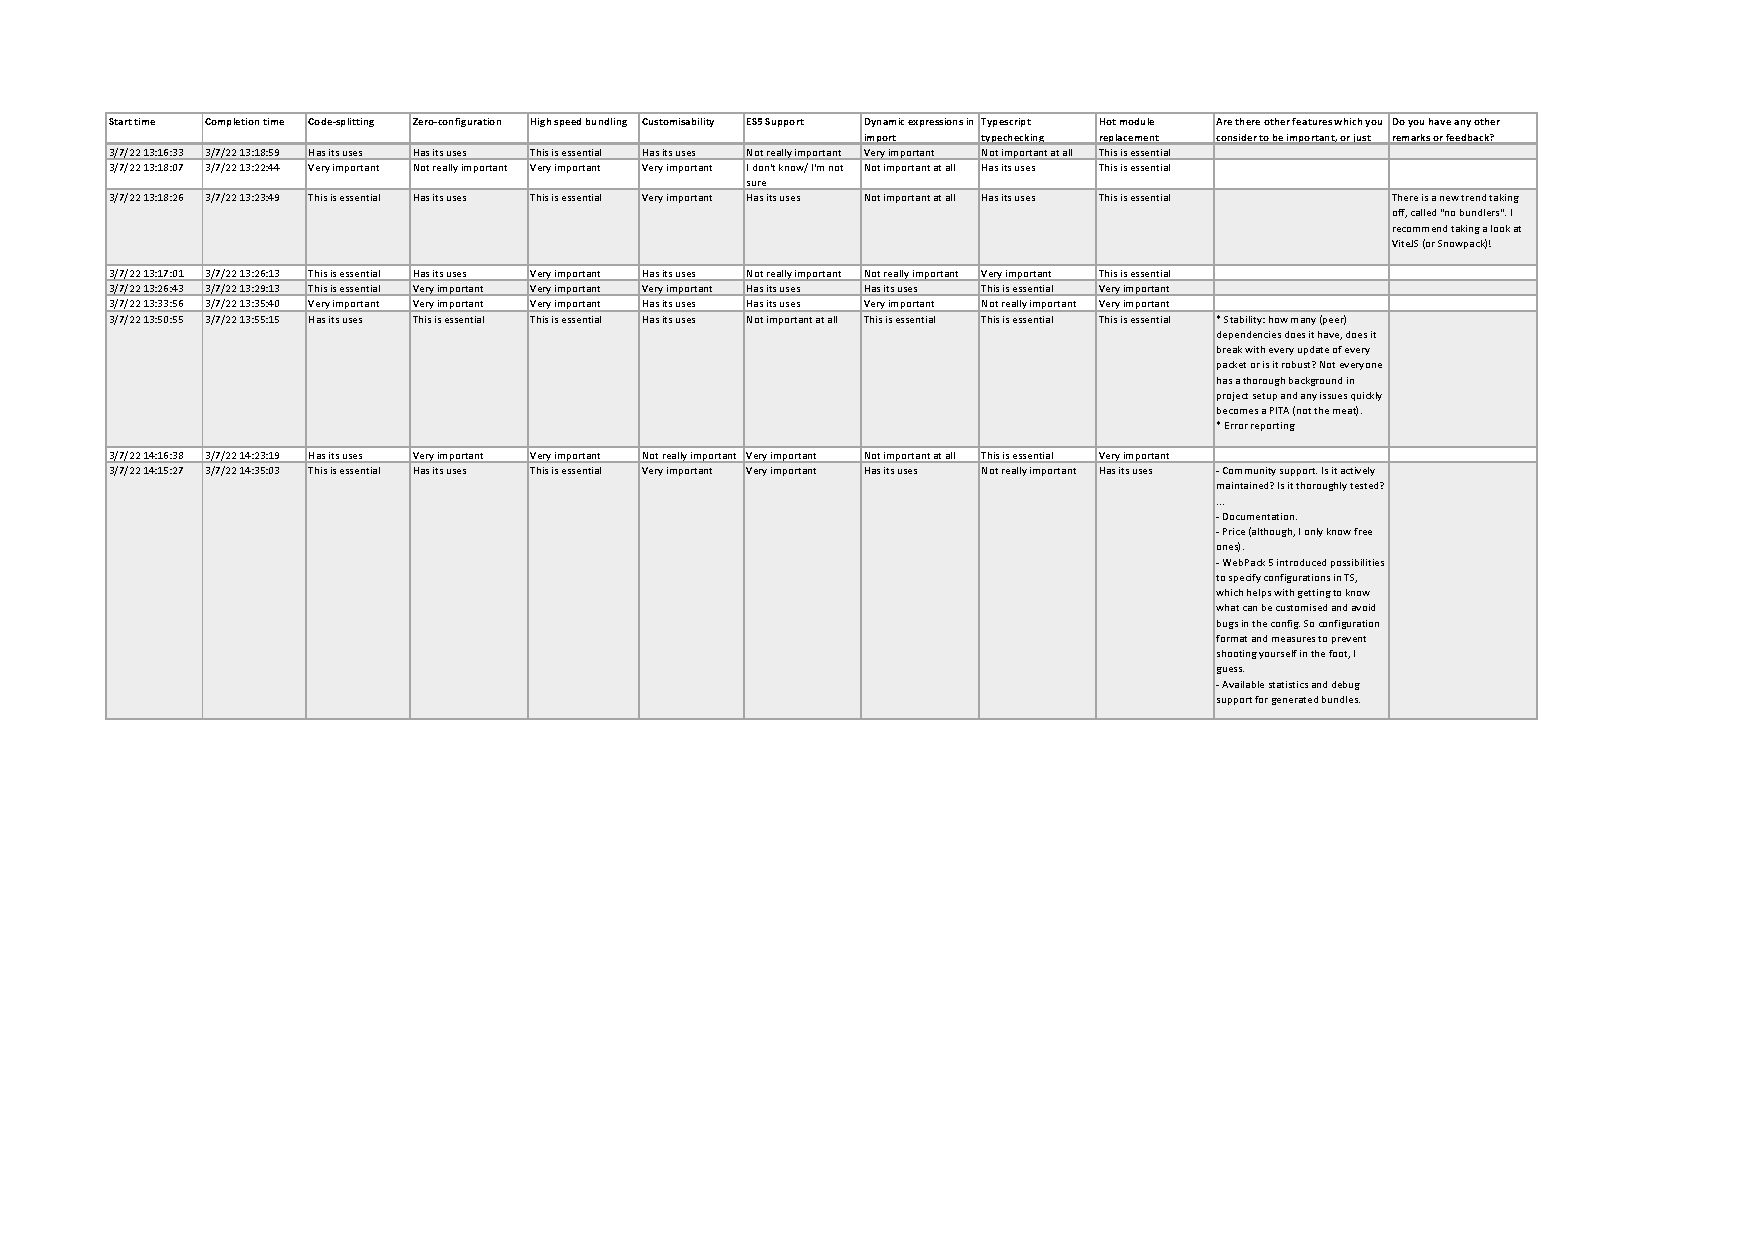
\includepdf[pages=1, landscape=true]{./appendix/survey-developers-questions.pdf}

\chapter{Resultaten Vragenlijst Developers}

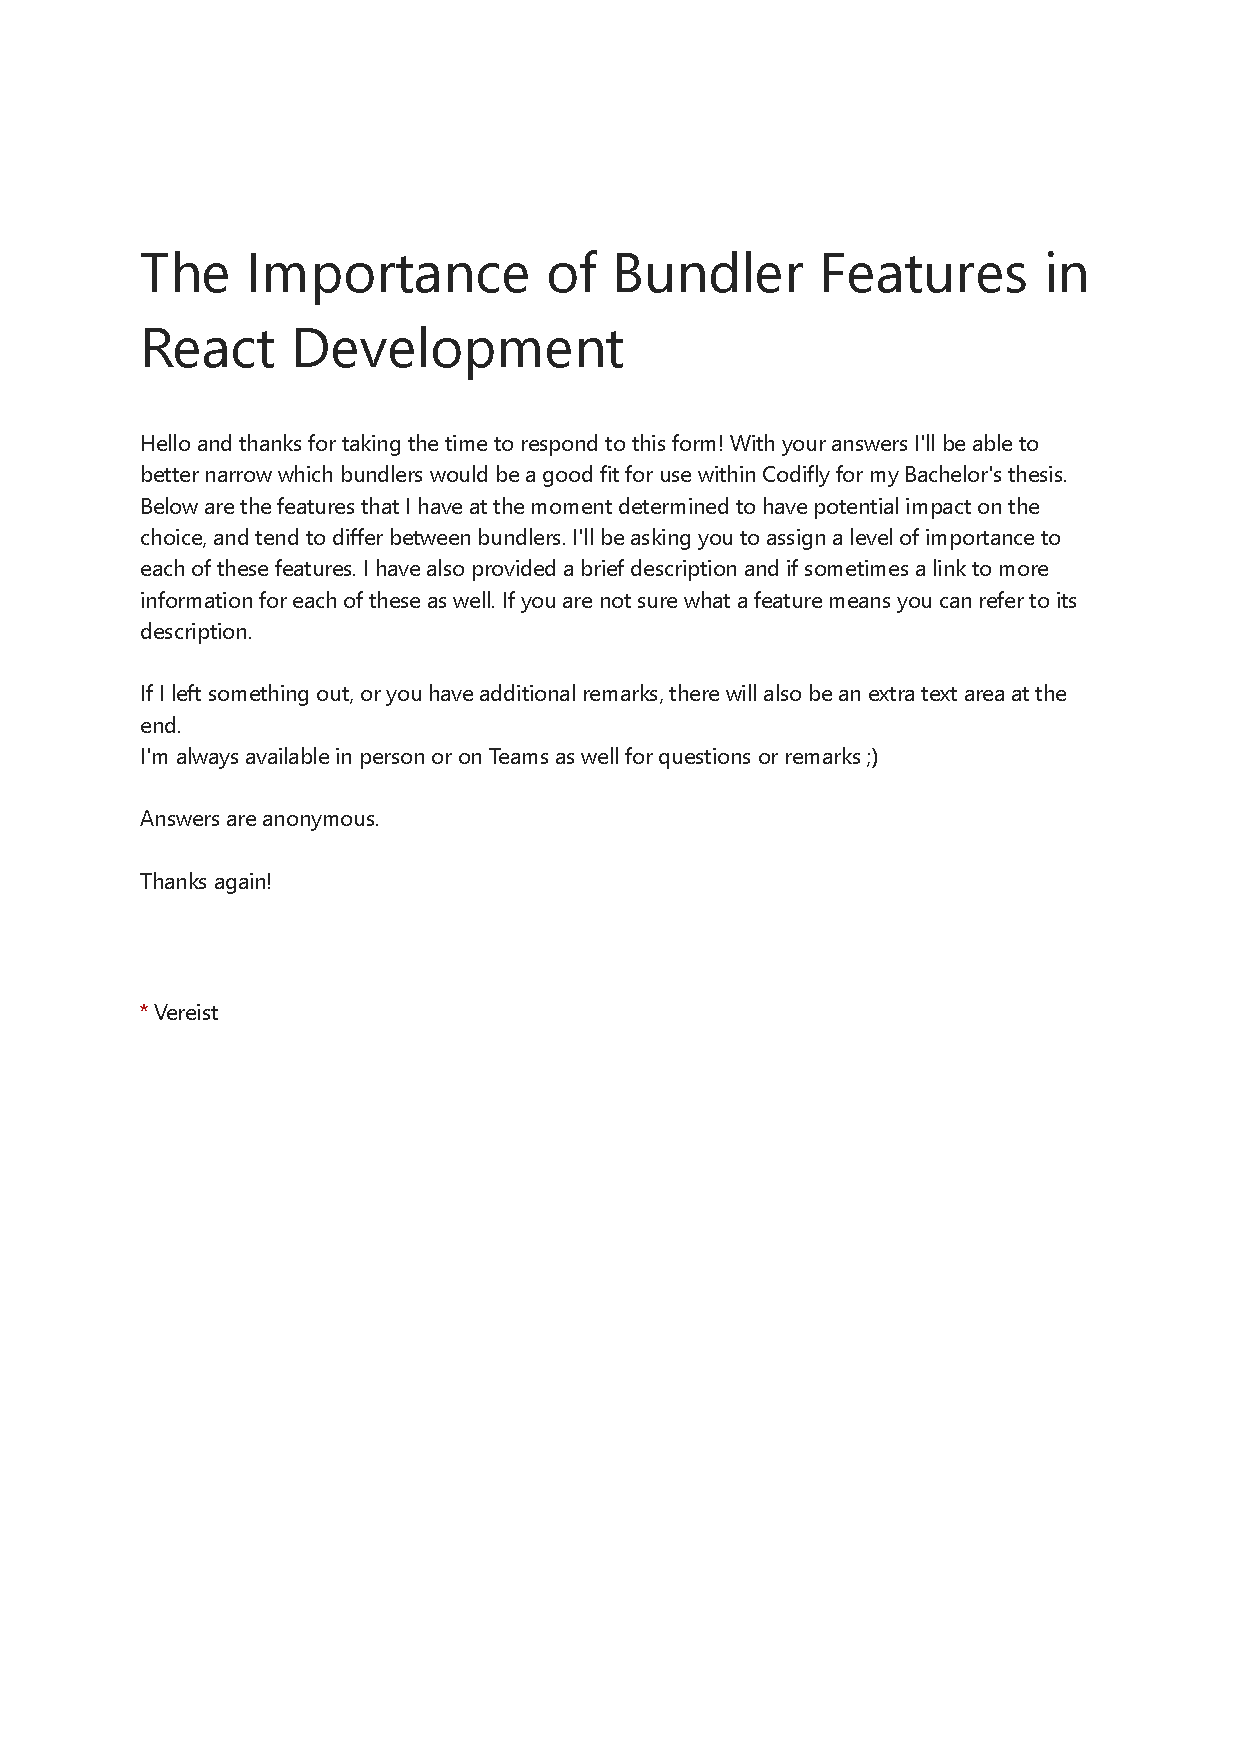
\includepdf[pages={1-4}]{./appendix/survey-developers-answers.pdf}

\chapter{Resultaten Benchmarks}
\label{appendix:benchmarks}

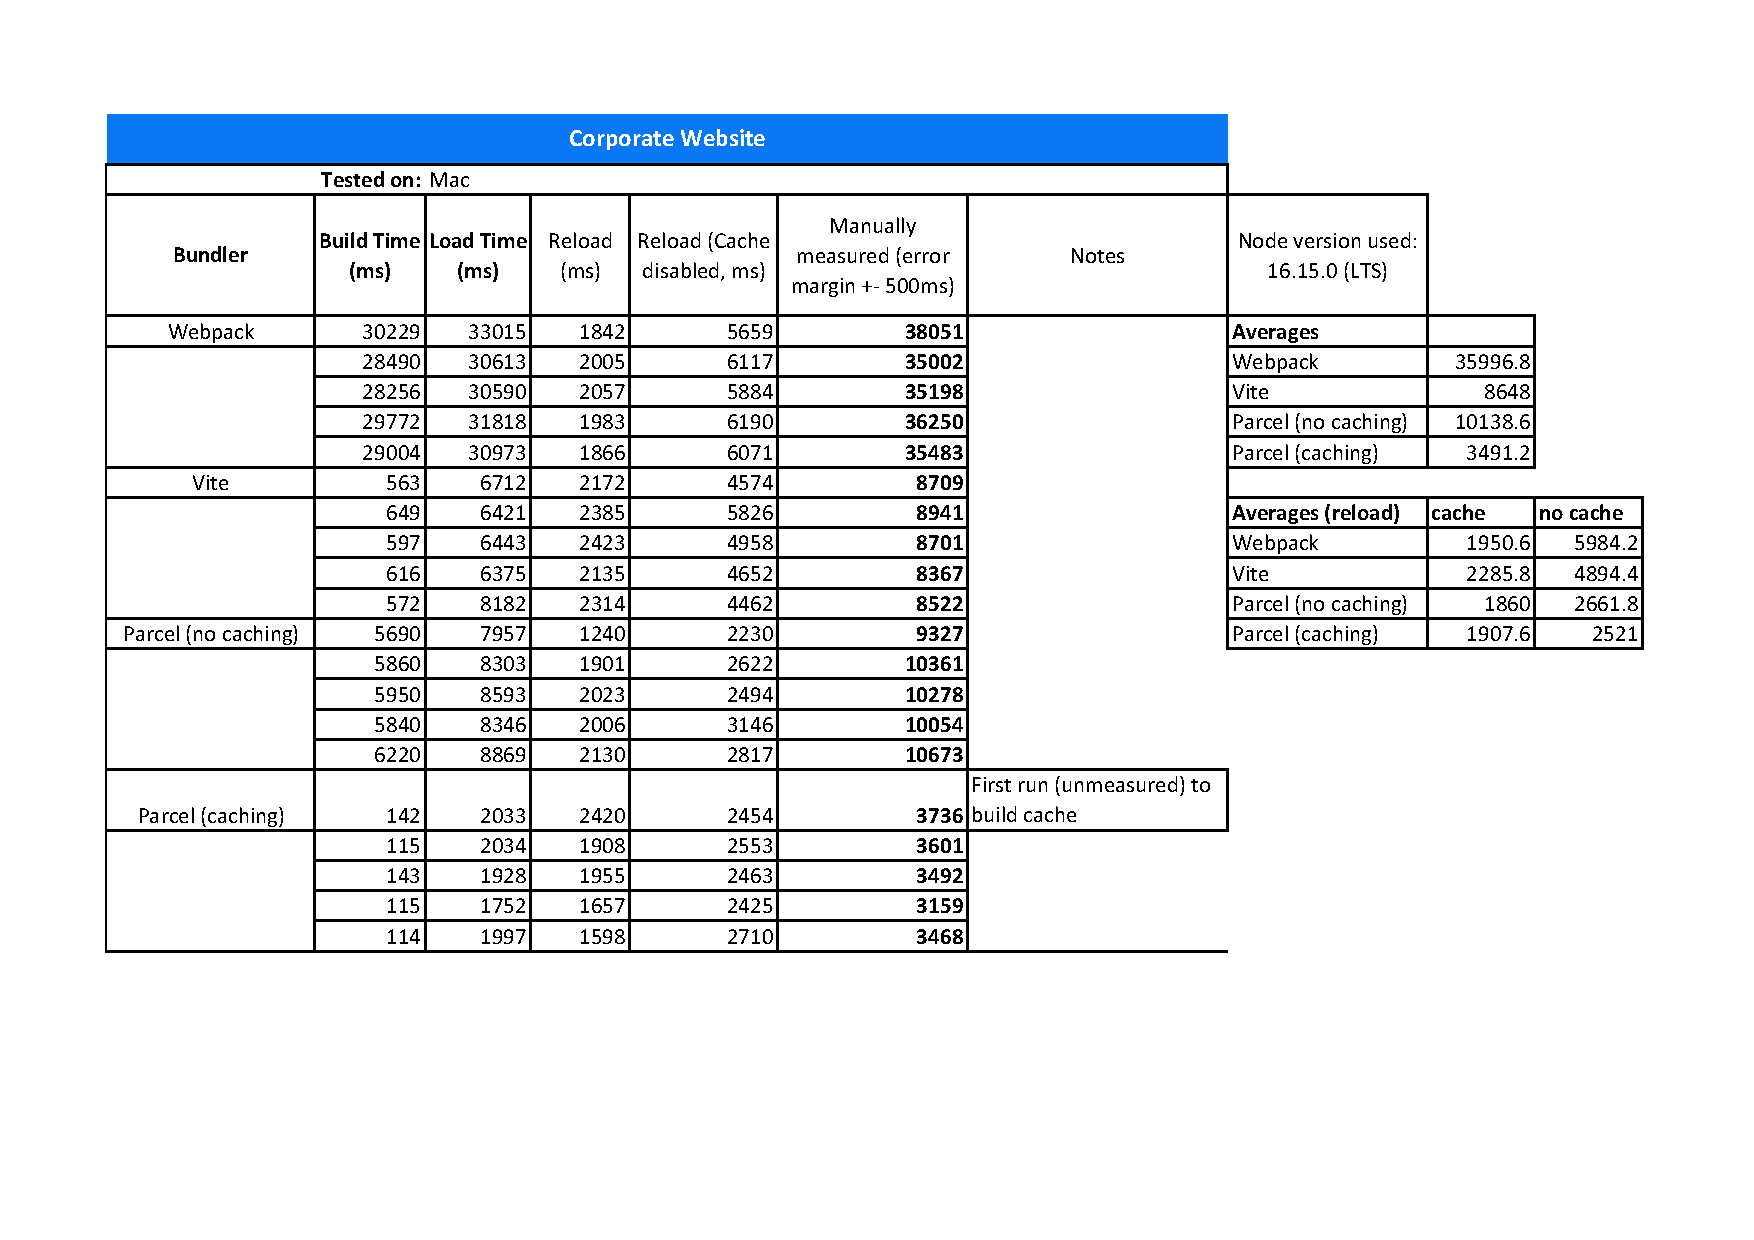
\includepdf[pages={1-3}]{./appendix/results.pdf}

%%---------- Onderzoeksvoorstel -----------------------------------------------

\chapter{Onderzoeksvoorstel}

Het onderwerp van deze bachelorproef is gebaseerd op een onderzoeksvoorstel dat vooraf werd beoordeeld door de promotor. Dat voorstel is opgenomen in deze bijlage.

% Verwijzing naar het bestand met de inhoud van het onderzoeksvoorstel
\setlength{\parskip}{0.2em}
%---------- Inleiding ---------------------------------------------------------

\section{Introductie} % The \section*{} command stops section numbering
\label{sec:introductie}
Dynamische webapplicaties zijn onmogelijk zonder een ondersteunende programmeertaal. Binnen Codifly en zeer veel andere bedrijven komt die in de vorm van JavaScript. Doorheen de jaren zijn veel hulpmiddelen gekomen en gegaan om de ontwikkelaars van zulke webapplicaties te ondersteunen. Van het omzetten van de ene taal naar de andere, tot automatische samenbundeling van je code. In deze paper zal gekeken worden naar verschillende TypeScript transpilers en JavaScript bundlers, om zo hopelijk te kunnen concluderen welke TypeScript transpilers en JavaScript bundlers het waard zijn om een oog op te houden, welke voor- en nadelen ze hebben, en of bepaalde combinaties een synergie hebben met elkaar bij ontwikkeling van React applicaties in het algemeen. Verder zal na het achterhalen van welke transpilers en bundlers Codifly momenteel in gebruik neemt er aan de hand van een proof-of-concept dan ook geanalyseerd kunnen worden welke mogelijke positieve invloed een andere keuze zou kunnen hebben binnen het ontwikkelingsproces van Codifly.

%---------- Stand van zaken ---------------------------------------------------

\section{State-of-the-art}
\label{sec:state-of-the-art}

\subsection{De limitaties van JavaScript}
Binnen het gebied van webontwikkeling wordt zeer vaak met JavaScript in contact gekomen. JavaScript heeft echter bepaalde limitaties die het ontwikkelingsproces kunnen hinderen. \autocite{geeksforgeeks_2021}

Alle programmeertalen zijn tot op een zekere mate zwak/sterk getypeerd, en dynamisch/statisch getypeerd. In een dynamisch getypte taal hebben alle waarden een type aan zich verbonden tijdens runtime\footnote{Wanneer de applicatie uitgevoerd wordt.}. JavaScript, een dynamisch getypte taal, houdt paren van een waarde en type bij; bijvoorbeeld (Number, 4). Een statisch getypte taal moet dit niet doen, aangezien we variabelen expliciet een type geven in onze broncode.

De mate waarin een taal sterk of zwak getypeerd is hangt af van hoe strikt de taal types afdwingt. De \lq type coercion \rq die een taal aanbiedt is hier een typisch voorbeeld van. Type coercion is het proces van het omzetten van waarden van het ene type naar het andere. Als men in JavaScript een variabele declareren als volgt:

\verb|const waarde = true + false|

Dan zal waarde het nummer 1 bevatten. JavaScript zet eerst de booleaanse waarden om naar nummers om ze op te tellen. Wat je gedaan hebt is dus effectief:

\verb|const waarde = 1 + 0|

In een sterk getypte taal zal dit veel strenger afgedwongen worden, maar de exacte limitaties hangen nog steeds van taal tot taal af. Welke soort typering het beste is, is geen eenzijdige discussie. Onderzoek van \textcite{meijer_drayton_2004} ondersteund de notie dat het gebruik van dynamische typering in een statisch getypte omgeving een gulden middenweg is.

\subsection{Exit JavaScript, enter TypeScript}

\subsubsection{De browser}
Om JavaScript uit te kunnen voeren in een browser, moet die browser een JavaScript engine hebben. Elke moderne browser heeft een JavaScript engine dat zich aan de ECMAScript standaard houdt. ECMAScript bestaat uit versies, en met elke nieuwe versie worden een aantal nieuwe JavaScript features ondersteund. Browserontwikkelaars implementeren echter niet in één keer de volledige versies van ECMAScript, maar werken feature per feature. Het resultaat hiervan is dat elke browser een andere set JavaScript features bevat. Op het moment van dit onderzoek ondersteunen alle major browsers ES6\footnote{ES is een afkorting van ECMAScript.}. Een vollediger overzicht van de relatie tussen JavaScript en ECMAScript, en het nut van ECMAScript wordt ook gedetailleerd in onderzoek van \textcite{olund_karlsson_2016}

\subsubsection{TypeScript in de browser}
Om TypeScript code gebruiksklaar te maken, moet ze dus eerst omgezet worden naar de JavaScript die onze browser wel begrijpt. Dit proces noemt transpilatie\footnote{De termen compilatie en transcompilatie worden ook vaak gebruikt. In de context van deze paper zijn ze alle drie synoniem met elkaar.}.

De transpilers die bekeken zullen worden in deze paper zijn als volgt:

\begin{itemize}
  \item TSC
  \item Babel
  \item SWC
  \item Sucrase
  \item ESBuild\footnote{ESBuild is eigenlijk een bundler, maar heeft ook ingebakken ondersteuning voor TypeScript transpilatie. \autocite{reilly_2021}}
\end{itemize}

Deze transpilers transpileren ook features die horen bij nieuwere ES versies naar code die compatibel is met een oudere versie. Zo genieten ontwikkelaars enerzijds van nieuwere features, maar kunnen die ook op alle major browsers gebruikt worden.

Elke transpiler heeft zijn voor- en nadelen. Babel bestaat als sinds 2014, en is qua populariteit de huidige leider. Hoge populariteit betekent meer contributie, en meer contributie is dan weer meer features en stabiliteit. Dit is iets waar moeilijk mee te concurreren is voor nieuwere transpilers. De nieuwere transpilers hebben echter één groot voordeel: Sinds 2014 is de technologie veel veranderd, en nieuwe projecten zijn niet gelimiteerd aan bestaande keuzes in technologie. SWC is daar één van de betere voorbeelden van. SWC is geschreven in Rust, en heeft mede door die keuze een enorme verbetering in compilatietijden. \autocite{kang_2020, khosravi_2020}

\subsection{Bundlers}

Om een React project leesbaar te houden, worden verschillende pagina's en/of componenten verdeeld over verschillende bestanden. Het zou echter inefficiënt zijn om alle verschillende bestanden apart in je browser in te laden. Daarom wordt er gebruik gemaakt van bundlers. Bundlers gaan al je JavaScript (en andere assets) samenbundelen om alles te combineren in één JavaScript bestand.

Met het uitbrengen van HTTP/2 is er echter een gulden middenweg geopend. Met HTTP/1.1 moest je browser synchroon verzoeken sturen op een verbinding, en browsers omzeilen die limitatie van HTTP/1.1 door typisch 6 verbindingen tegelijk te maken met de webserver. Dit had wel één groot nadeel, met name het feit dat elke verbindingen die geopend wordt een overhead heeft: De TCP-connectie aanmaken, HTTPS handshake uitvoeren, het beheren van alle gelijktijdige verbindingen ... Met HTTP/2 is dit geen probleem meer. HTTP/2 staat toe om al je verzoeken gelijktijdig te maken op één verbinding. \autocite{hsu_2017} Op figuur \ref{fig:HttpComparison} wordt het verschil tussen de twee visueel voorgesteld.

HTTP/2 zorgt er als gevolg voor dat men eigenlijk niet alles moet bundelen in één bestand. Gebruik van Webpacks \lq AggressiveSplittingPlugin \rq met Reacts \lq @loadable/component \rq maken hier goed gebruik van om componenten efficiënt te lazy-loaden met gebruik van HTTP/2. \autocite{fraser_2020}

\begin{figure*}[!htp]
  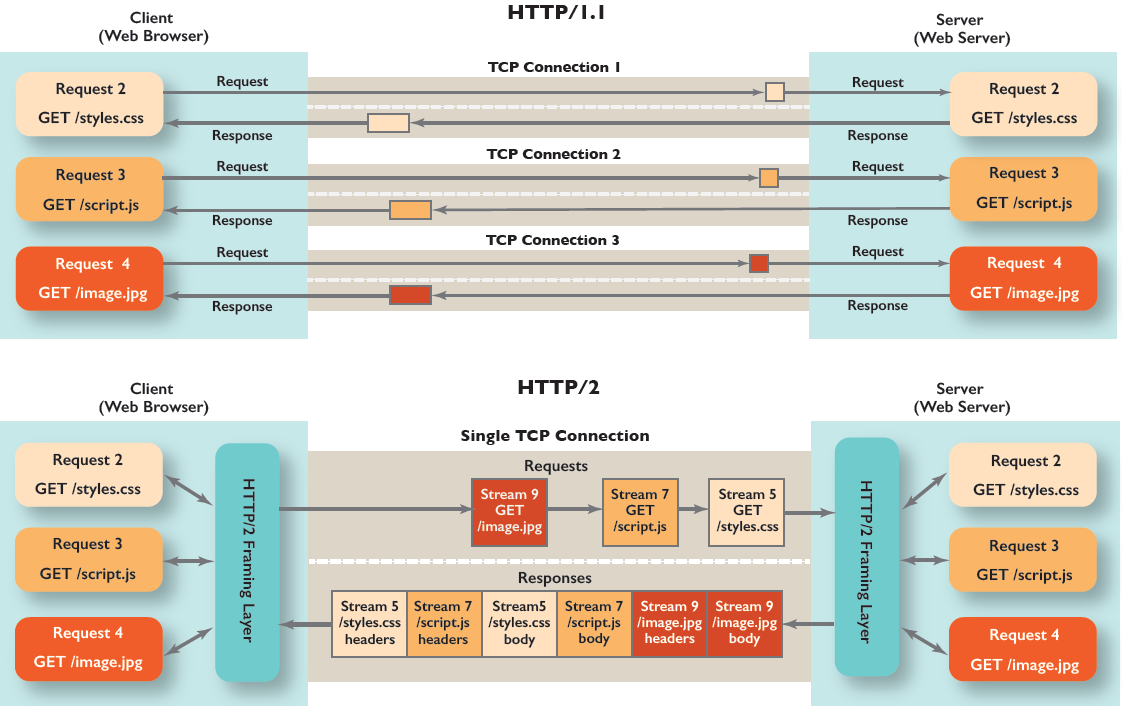
\includegraphics[width=\linewidth]{http.png}
  \caption{Visuele voorstelling van het verschil tussen het proces van een HTTP/1.1 en HTTP/2 verzoek, gemaakt door \cite{pollard_2018}}
  \label{fig:HttpComparison}
\end{figure*}

De bundlers die bekeken zullen worden in deze paper zijn als volgt:

\begin{itemize}
    \item Webpack
    \item ESBuild
    \item Vite
    \item Parcel
    \item Rollup
\end{itemize}

% Voor literatuurverwijzingen zijn er twee belangrijke commando's:
% \autocite{KEY} => (Auteur, jaartal) Gebruik dit als de naam van de auteur
%   geen onderdeel is van de zin.
% \textcite{KEY} => Auteur (jaartal)  Gebruik dit als de auteursnaam wel een
%   functie heeft in de zin (bv. ``Uit onderzoek door Doll & Hill (1954) bleek
%   ...'')


%---------- Methodologie ------------------------------------------------------
\section{Methodologie}
\label{sec:methodologie}

De transpilers en bundlers zullen beoordeeld worden gebaseerd op volgende criteria:

\begin{itemize}
  \item Snelheid
  \item Gebruiksvriendelijkheid
  \item Functionaliteit
  \item Huidige marktdominantie
\end{itemize}

Om de snelheid te beoordelen zullen voor elke transpiler en bundler benchmarks opgesteld worden aan de hand van met TypeScript opgestelde React applicaties van variërende groottes. De resultaten van deze benchmarks zullen geanalyseerd en vergeleken worden. Deze methodologie is geïnspireerd uit de methodes gebruikt in de analyse van \textcite{eaton_2021}. Vergeleken met de vooraf genoemde analyse, zullen hier meer nog pakketten vergeleken worden. Ook de reeds verkregen resultaten van die analyse zullen vergeleken kunnen worden met de resultaten van dit onderzoek.

Gebruiksvriendelijkheid zal beoordeeld worden aan de hand van een anonieme steekproef voor React developers, waar hun ervaringen met de transpilers en bundlers verzameld zullen worden.
De informatie die de onderzoeker tracht te achterhalen bevindt zich in tabel \ref{table:1}.
Ook overige externe bronnen die de gebruiksvriendelijkheid van deze pakketten bespreken kunnen gebruikt worden in de literatuurstudie om te helpen een duidelijkere conclusie te maken. Door de subjectieve aard van dit criterium is het alsnog ook mogelijk dat de eindconclusie van dit onderzoek er weinig of niet door beïnvloed zal worden. Dit zal worden bepaald door de onderzoeker aan de hand van de resultaten van de vragenlijst. De resultaten zullen echter hoe dan ook toegelicht worden.

\begin{table}[ht]
\begin{tabular}{|p{56mm}|l|}
\hline
\multicolumn{2}{|c|}{\textbf{Onafhankelijke variabelen}}         \\ \hline
\textbf{Variabele}                         & \textbf{Meetniveau} \\ \hline
Welke frameworks/libraries worden in de werkomgeving gebruikt& Nominaal\\ \hline
Gekende bundlers/transpilers               & Nominaal            \\ \hline
Uren ervaring per bundler/transpiler die in het laatste jaar gebruikt is& Ratio\\ \hline
Geobserveerde gebruiksvriendelijkheid per gebruikte bundler/transpiler& Ordinaal\\ \hline
Meest passende positieve kenmerk per gebruikte bundler/transpiler& Nominaal\\ \hline
Meest passende negatieve kenmerk per gebruikte bundler/transpiler& Nominaal\\ \hline
Eerste keuze bundler en transpiler in een nieuw project& Nominaal\\ \hline
Best-to-worst rangschikking van de gebruikte bundlers/transpiler& Ordinaal\\ \hline
\end{tabular}
\caption{Tabel van de informatie die achterhaalt tracht te worden door de vragenlijst.}
\label{table:1}
\end{table}

Functionaliteit wordt beoordeeld in het perspectief van React ontwikkeling. Missende of extra functionaliteit die een meerwaarde biedt aan ontwikkeling binnen React zal hier van het grootste belang zijn.

Marktdominantie zal gepeild worden aan de hand van data beschikbaar op NPM\footnote{Node Package Manager, ook gekend als NPM is de grootste repository voor JavaScript libraries}. Marktdominantie heeft onder andere een invloed op de ondersteuning van de onderhouders, de kwaliteit en kwantiteit van documentatie, en hoe waarschijnlijk het is dat een ontwikkelaar voorkennis heeft van de package.

Verder zal er ook aan de hand van praktische proeven bekeken worden welke transpilers en bundlers een eventuele goede samenwerking hebben met elkaar. Het is immers mogelijk dat één transpiler zich vestigt als de snellere, terwijl een tegenhanger veel betere samenwerking heeft met een bepaald bundler. Dit kan tot verandering leiden in de eindconclusie.

Om de beste combinaties tussen bundler en transpiler te identificeren binnen Codifly, zal er een individuele bevraging gebeuren om hun noden en prioriteiten vast te leggen.

Ten slotte zal een proof-of-concept opgesteld worden om de als best beschouwde combinatie in het spotlicht te zetten, en zo aan te tonen dat die combinatie aan te raden valt voor regelmatig gebruik binnen Codifly indien dit niet reeds het geval is.

%---------- Verwachte resultaten ----------------------------------------------
\section{Verwachte resultaten}
\label{sec:verwachte_resultaten}

\begin{figure*}[!htp]
  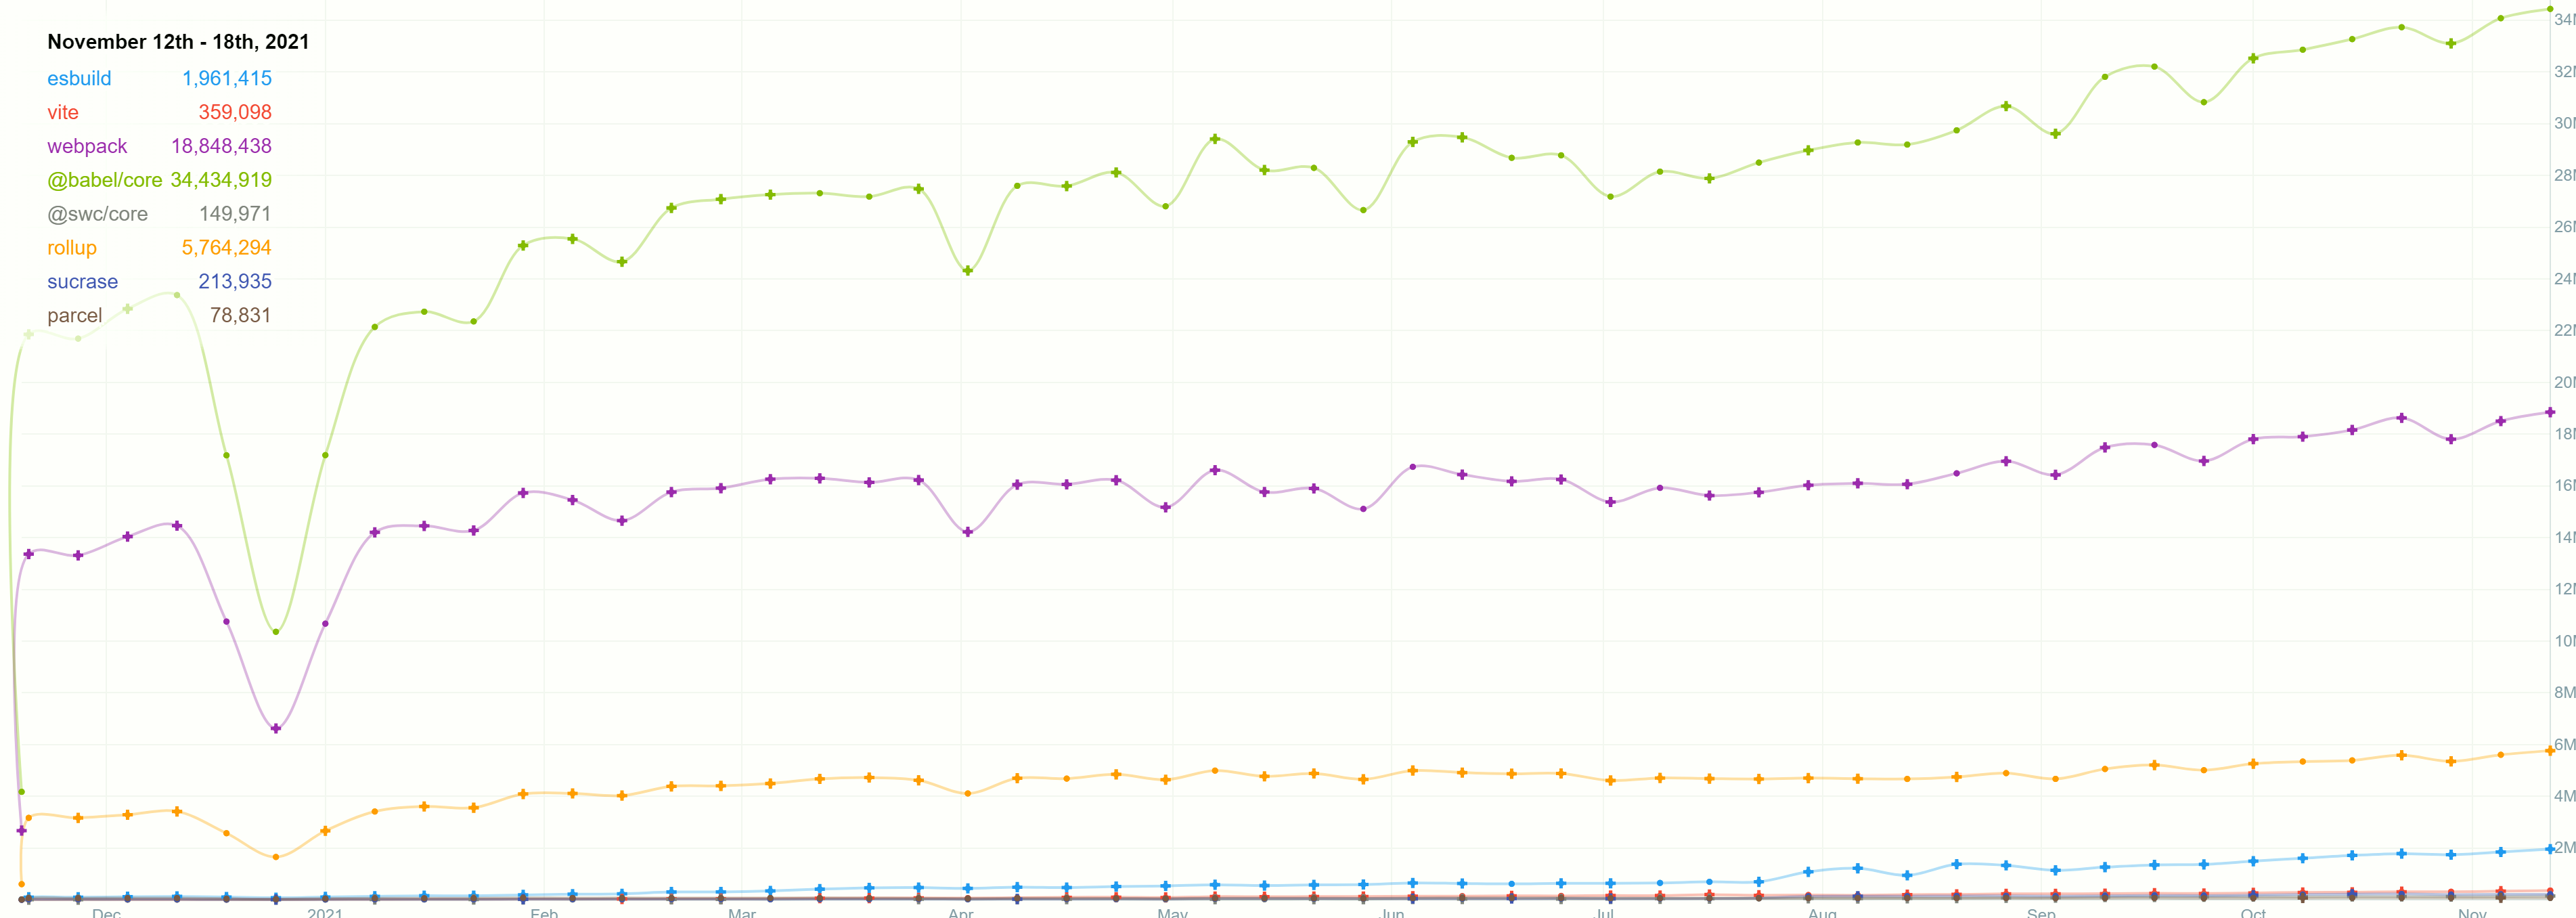
\includegraphics[width=\linewidth]{npmgraph.png}
  \caption{Lijndiagram van het aantal downloads van alle te onderzoeken bundlers en transpilers, behalve TSC. TSC is ingebouwd in TypeScript.}
  \label{fig:NpmDownloadsLineChart}
\end{figure*}

Populaire opties zoals bijvoorbeeld Babel en Webpack zijn niet altijd de snelste, maar hebben meer documentatie om mee te werken. Het is dan ook verwacht dat populairdere transpilers en bundlers eerder naar de gebruiksvriendelijke kant zullen leunen, terwijl de jongere en volop groeiende transpilers en bundlers sneller zullen zijn. Maar mogelijks met het nadeel van minder, of minder duidelijke documentatie. Uit figuur \ref{fig:NpmDownloadsLineChart} kunnen de populariteitstrends voor bijna alle transpilers en bundlers geïdentificeerd worden, wat hoogstwaarschijnlijk in de steekproef gereflecteerd zal worden.

%---------- Verwachte conclusies ----------------------------------------------
\section{Verwachte conclusies}
\label{sec:verwachte_conclusies}

Elke bundler en transpiler heeft een licht verschillende set van doelen die de maintainers willen bereiken. Er is dan echter ook waarschijnlijk geen één beste keuze die gemaakt kan worden op algemeen vlak. Binnen Codifly moet echter eerst achterhaald worden waar hun prioriteiten liggen bij de keuze van transpiler en bundler. Afhankelijk van de ondervindingen zal het antwoord nog veel kunnen variëren. 

De onderzoeker verwacht dat de rijpere projecten enige voorkeur zullen hebben, omwille van het feit dat die momenteel al in gebruik zijn, een goede basis hebben aan documentatie en een vollediger arsenaal hebben aan features.

Verder is er ook enige onzekerheid of dit onderzoek een werkelijk betere optie zal kunnen formuleren voor Codifly. Wanneer frameworks zoals Next.js in gebruik genomen worden is het ook niet altijd zo simpel om de bijgeleverde bundler en transpiler zomaar te vervangen. Voor projecten waar echter niet gebruik gemaakt wordt van een React framework zou dit niet het geval zijn.


%%---------- Andere bijlagen --------------------------------------------------
% TODO: Voeg hier eventuele andere bijlagen toe
%\input{...}

%%---------- Referentielijst --------------------------------------------------

\printbibliography[heading=bibintoc]

\end{document}
